\documentclass[12pt,a4paper]{article}

\usepackage[utf8]{inputenc}
\usepackage{polski}
\usepackage[polish]{babel}

\usepackage{microtype}
\DisableLigatures{encoding = *, family = *}

\usepackage[left=2.5cm, right=2.5cm, top=2.5cm, bottom=2.5cm]{geometry}
\usepackage{indentfirst}

\usepackage{graphicx}

\begin{document}
	
		\begin{titlepage}

		\vspace*{1cm}

	    \begin{center}
		    \small
		    Politechnika Wrocławska\\
		    Wydział Elektroniki\\
		    Podstawy Technik Mikroprocesorowych
	    \end{center}

	    \vspace{3cm}

		\noindent\rule{\linewidth}{0.4mm}
	    \begin{center}
			\LARGE \textsc{Mikroprocesorowy Sterownik Śledzący Anteny Satelitarne} !!!!
	    \end{center}
		\noindent\rule{\linewidth}{0.4mm}

		\vspace{0.5cm}

%Do poprawienia na pierwszej stronie.
%http://en.wikibooks.org/wiki/LaTeX/Title_Creation
	    \begin{flushright}
			\begin{minipage}{6cm}
				\textit{\small Autor:}\\
				\normalsize \textsc{Paweł Szwagierek}
			\end{minipage}
			\vspace{3cm}
			{\small Prowadzący:}\\
			dr inż. Jerzy Greblicki
	    \end{flushright}

	    \vspace*{\stretch{6}}

	    \begin{center}
		    \today
	    \end{center}	
    \end{titlepage}


	\tableofcontents
	\clearpage

	\section{Wstęp}
	Celem projektu jest zbudowanie sterownika rotora antenowego dla zastosowań krótkofalarskich. Sterownik mikroprocesorowy powinien umieć skierować antenę w ustalonym kierunku według podanych współrzędnych horyzontalnych (Azymut i Elewacja).

	\section{Protokół DDE}

	\section{Przygotowanie oprogramowania po stronie komputera}
		
		\subsection{Konfiguracja programu Orbitron}
		Koniecznymi ustawieniami w programie Orbitron są:
		\begin{enumerate}
			\item Współrzędne geograficzne położenia anteny
			\item Wysokość nad poziomem morza (konieczna do korekcji elewacji)
			\item Wybór sterownika DDE
		\end{enumerate}

			\subsubsection{Współrzędne geograficzne oraz wysokość nad poziomem morza}
			Współrzędne geograficzne oraz wysokość ustawia się w zakładce Lokalizacja przedstawionej na rysunku~\ref{fig:location_settings}. Długość i szerokość geograficzną można wpisać ręcznie w pola tekstowe lub wybrać z już zdefiniowanych profili. Wysokość nad poziomem morza należy wpisać ręcznie w pole tekstowe. Po ustawieniu koniecznych opcji lokalizacji, konfigurację można zapisać na liście konfiguracji prywatnych.

			\begin{figure}[!htb]
				\begin{center}
					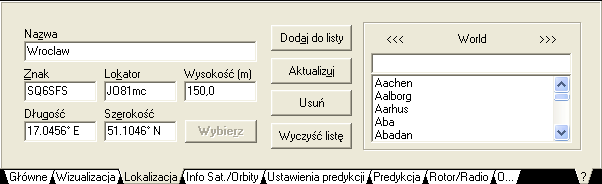
\includegraphics[scale=0.7]{screen1}
				\end{center}
				\caption{Orbitron - Ustawienia lokalizacji}
				\label{fig:location_settings}
			\end{figure}

			\subsubsection{Wybór sterownika DDE}
			Do komunikacji programu Orbitron ze światem zewnętrznym - a w szczególności ze sterownikiem antenowym - konieczym jest użycie zewnętrznego sterownika do transmisji danych (DDE). W tym wypadku użyty został sterownik WispDDE. Należy go wybrać z listy sterowników w zakładce Rotor/Radio programu Orbitron tak jak to jest widoczne na rysunku~\ref{fig:DDE_settings}. Po dokonaniu wyboru, należy kliknąć przycisk znajdujący się obok listy uruchamiający sterownik. Może się zdarzyć, że program Orbitron nie będzie mógł zlokalizować sterownika na komputerze i poprosi o ręczne wskazanie jego położenia na dysku.
			
			\begin{figure}[!htb]
				\begin{center}
					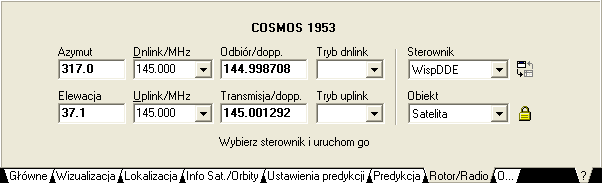
\includegraphics[scale=0.7]{screen2}
				\end{center}
				\caption{Orbitron - Ustawienia sterownika DDE}
				\label{fig:DDE_settings}
			\end{figure}

		\subsection{Konfiguracja sterownika DDE}
		\begin{figure}[!htb]
			\begin{center}
				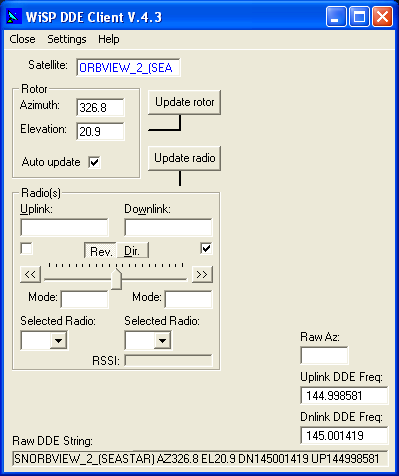
\includegraphics[scale=0.7]{screen3}
			\end{center}
			\caption{WispDDE - Główne okno programu}
			\label{fig:WispDDE_main_window}
		\end{figure}
		Po uruchomieniu sterownika przez program Orbitron, należy przeprowadzić jego krótką, wstępną konfigurację. Po pojawieniu się głównego okna programu pokazanego na rysunku~\ref{fig:WispDDE_main_window} należy sprawdzić, czy sterownik poprawnie odebrał dane od programu Orbitron i wyświetlił nazwę wybranej satelity. Następnie z menu \texttt{Settings} wybieramy okno \texttt{DDE Link} przestawione na rysunku~\ref{fig:WispDDE_DDE_Link_settings} i wybieramy takie same opcje. 
		\begin{figure}[!htb]
			\begin{center}
				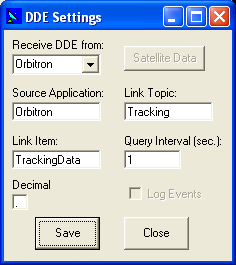
\includegraphics[scale=0.5]{screen4}
			\end{center}
			\caption{WispDDE - Okno konfiguraji DDE Link}
			\label{fig:WispDDE_DDE_Link_settings}
		\end{figure}
		Po zapisaniu tych ustawień, przechodzimy do kolejnego okna ustawień sterownika DDE wybierając z menu \texttt{Settings} pozycję \texttt{Rotor}. W tym oknie należy wybrać opcję interfejsu komunikacyjnego, portu oraz szybkości transmisji jak na rysunku~\ref{fig:WispDDE_Rotor_settings}. Konfiguracja użyta w projekcie to:
		\begin{description}
			\item[Interface Type] GS-232
			\item[Port] COM1
			\item[Baud Rate] 9600
		\end{description}
		
		\begin{figure}[!htb]
			\begin{center}
				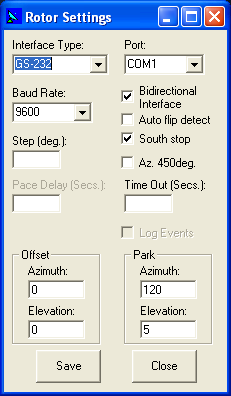
\includegraphics[scale=0.5]{screen5}
			\end{center}
			\caption{WispDDE - Okno konfiguraji Rotor}
			\label{fig:WispDDE_Rotor_settings}
		\end{figure}

	\section{Przygotowanie środowiska}

		\subsection{Mikrokontroler STM32F0 - Discovery}
		Przed podłączeniem mikrokontrolera do komputera w celu jego programowania należy zainstalować jego sterowonik w systemie operacyjnym. W tym celu należy zainstalować dołączony do projektu plik ST-Link Driver. Następnie po podłączeniu mikrokotrolera do komputera pojawi się okno instalacji jego sterownika, należy wyrazić zgodę na jego instalację w systemie. Gdyby okno instalacji sterownika nie pojawiło się po podłączeniu miktokontrolera, należy w systemowym Menadżerze urządzeń wybrać niezainstalowane urządzenie i wybrać opcję aktualizacji jego sterownika.

	\section{Wnioski oraz podsumowanie}
	***WWW***

	\clearpage
	\listoffigures

	\vfill
	\hfill Dokumentacja przygotowana w \LaTeXe

\end{document} %End of document.